\documentclass[tikz,border=3.14pt]{standalone}
\usepackage{amsmath}
\usetikzlibrary{3d,decorations.text,shapes.arrows,positioning,fit,backgrounds,arrows}
\usepackage{caption}

\captionsetup[table]{labelformat=empty}

\begin{document}

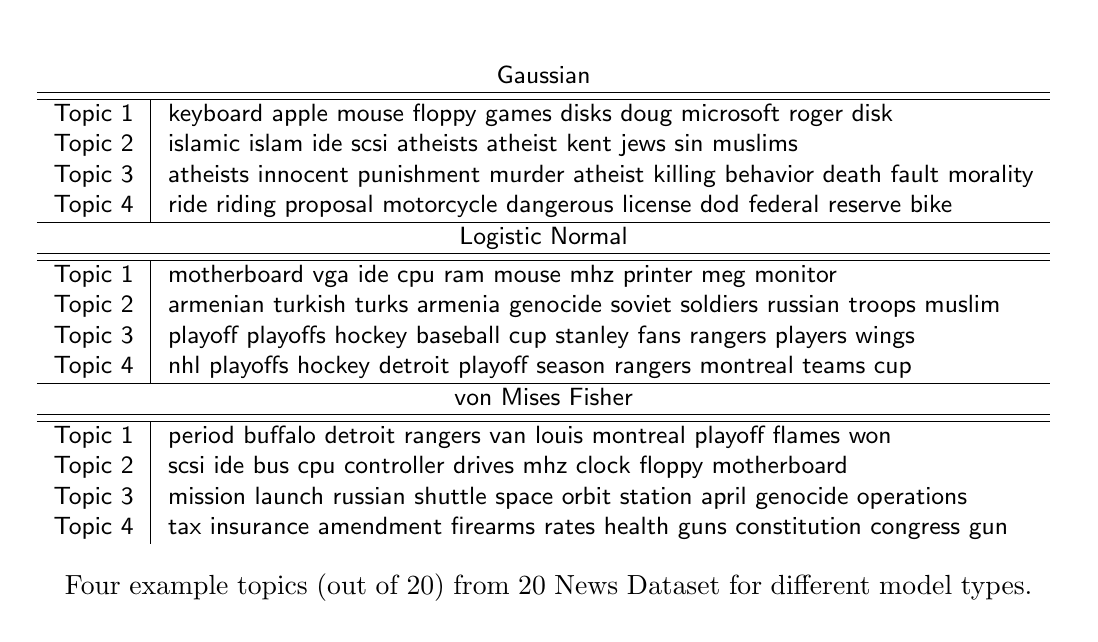
\begin{tikzpicture}[font=\sffamily\small,scale=2]

\node[text width=13cm] at (0,0) {
  \begin{table}[]
    \begin{tabular}{l|l}
      \multicolumn{2}{c}{Gaussian} \\
      \hline
      \hline
      Topic 1 & keyboard apple mouse floppy games disks doug microsoft roger disk \\
      Topic 2 & islamic islam ide scsi atheists atheist kent jews sin muslims \\
      Topic 3 & atheists innocent punishment murder atheist killing behavior death fault morality \\
      Topic 4 & ride riding proposal motorcycle dangerous license dod federal reserve bike \\
      \hline
      \multicolumn{2}{c}{Logistic Normal} \\
      \hline
      \hline
      Topic 1 & motherboard vga ide cpu ram mouse mhz printer meg monitor \\
      Topic 2 & armenian turkish turks armenia genocide soviet soldiers russian troops muslim \\
      Topic 3 & playoff playoffs hockey baseball cup stanley fans rangers players wings \\
      Topic 4 & nhl playoffs hockey detroit playoff season rangers montreal teams cup \\
      \hline
      \multicolumn{2}{c}{von Mises Fisher} \\
      \hline
      \hline
      Topic 1 & period buffalo detroit rangers van louis montreal playoff flames won \\
      Topic 2 & scsi ide bus cpu controller drives mhz clock floppy motherboard \\
      Topic 3 & mission launch russian shuttle space orbit station april genocide operations \\
      Topic 4 & tax insurance amendment firearms rates health guns constitution congress gun      
    \end{tabular}
    \caption*{Four example topics (out of 20) from 20 News Dataset for different model types.}
  \end{table} };

\end{tikzpicture}
\end{document}
  
